\chapter{DC Voltage Generation}
\label{ch:references}
\begin{comment}
Video 19

* start from AC (110V/220V, 50/60 Hz) -> generate DC
* ideal DC: keep Rin as low as possible
* From 220V to lower: use transformer
* From AC to DC: (1) use diode as in slide 30
* quid power losses ? -> loss of 60-70\%
* + diode needs 0.6 V (better: Ge diodes: smaller gap (.3V))
* improve with Graetz cell (redraw ...) -> avergage ~60 \%

Video 20
* From Graetz cell: fully-rectified signal (^^^^^^) but lose 2x 0.6
* with capacitor: filter waveform with RC filter
* charge duringe delta via diode
* after maximum: discharge of C through load (C provides current)
\end{comment}


The problem we address in this chapter is the generation of a fixed DC voltage of arbitrary value, without too much variation (\emph{ripple}). The supply we have at our disposal is the local AC voltage, which can have a value of 110 V, 210 V or 220 V, and a frequency of 50 Hz or 60 Hz, depending on where you are in the world.

\begin{minipage}{.5\textwidth}
	\centering
	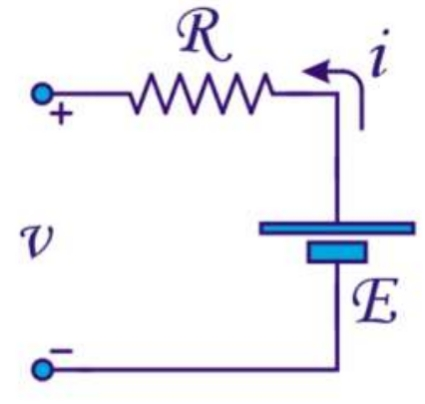
\includegraphics[width=4cm]{figures/ch12/dc_source1.jpg}
	\captionof{figure}{}
	\label{fig:dc_source1}
\end{minipage}%
\begin{minipage}{.5\textwidth}
	\centering
	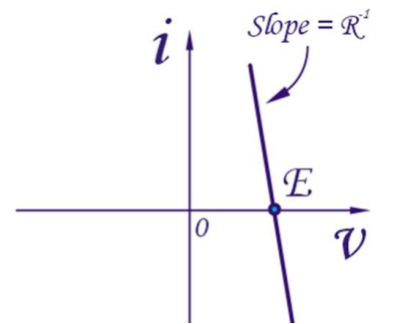
\includegraphics[width=5cm]{figures/ch12/dc_source2.jpg}
	\captionof{figure}{}
	\label{fig:dc_source2}
\end{minipage}

An ideal DC voltage source does not exist: every source will have an internal impedance $R$ as in figure \ref{fig:dc_source1} such that the generated voltage will decrease with the current drawn from the source as in figure \ref{fig:dc_source2}. In an ideal source, the load line would be a vertical line. Furthermore, every source will exhibit a ripple: there will be variations around an average value of the output voltage, even if the load stays the same. Our goal is to implement a DC power supply, generated from an available AC power supply, with minimum ripple $e$ and a low internal impedance.\\
We will do this in couple of steps. First, the voltage of the AC supply will be converted with a transformer to a level that is more suited. Then, a rectifier, together with a low-pass filter will be used to generate a DC voltage that still has a significant ripple. This ripple will be (partially) removed by using a voltage stabilizer.

\section{AC voltage modification}
Our first task is to modify (reduce) the AC voltage: we try to transfer from $220$ V to closer to a voltage that we need (about $\sim 10$'s of Volts). This can easily be done by using a transformer, as in figure \ref{fig:transformer1}. By setting the turns ratio $n$, we obtain a smaller amplitude:
$$
v_o = \frac{v_i}{n}
$$
and the current through the load is $i_o = n \; i_i$, i.e. the power through the load $v_o(t) \; i_o(t) = v_i(t) \; i_i(t)$ is preserved. However, losses can occur and the efficiency decreases for higher powers or currents.
	
\begin{figure}[h!]
	\centering
	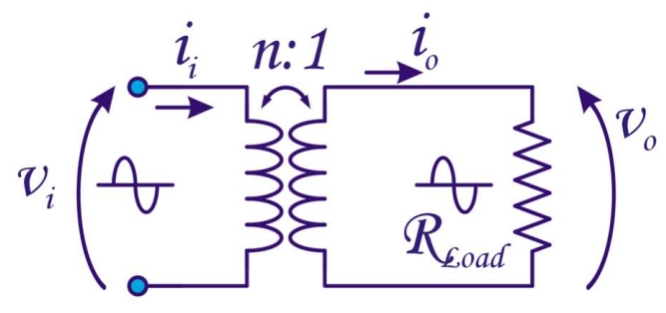
\includegraphics[width=8cm]{figures/ch12/transformer1.jpg}
	\caption{}
	\label{fig:transformer1}
\end{figure}

\section{Diode Rectifier}
\label{sec:diode_rectifier}
To transform an AC signal to a DC signal, we first try by using a diode as rectifier as in figure \ref{fig:rectifier1}. In this way, there will only be a current $i_o$ when $v_i > 0$.
\begin{figure}[h!]
	\centering
	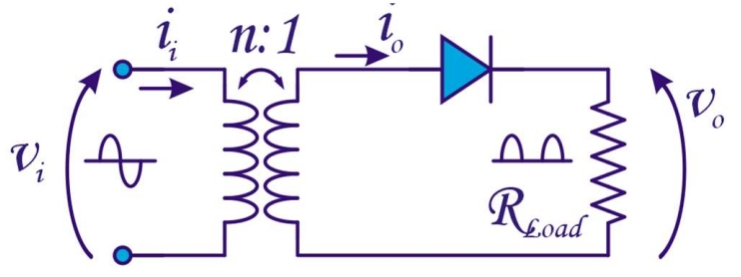
\includegraphics[width=8cm]{figures/ch12/rectifier1.jpg}
	\caption{}
	\label{fig:rectifier1}
\end{figure}
We can compute the average output current:
$$
I_{CC} = \frac{1}{T} \int_{t=t_0}^{t_0 + T} i_{Load}(t) \; dt = \frac{1}{T} \int_{t=t_0}^{t_0 + T/2} I_m \sin(\omega t) \; dt = \frac{I_m}{\pi} = \frac{V_m}{\pi \; R_{Load}} \approx 32\%  \frac{V_m}{R_{Load}} 
$$
This means that we lose more than 60\% of the output voltage swing. Additionally, we also lose one diode threshold voltage. A potential improvement is to use a germanium diode instead of silicon, because of the lower threshold voltage.\\
An improvement that allows conduction during both parts of the cycle, is the \emph{Graetz cell} in figure \ref{fig:graetz}. During the positive part of the cycle, the two horizontal diodes conduct; during the negative part the diagonal diodes will conduct. So there is a current through the load during the entire cycle and this current always flows in the same direction. We can compute the DC current, as before:
$$
I_{CC} = \frac{1}{T} \int_{t=t_0}^{t_0 + T} i_{Load} \; dt = \frac{2}{T} \int_{t=t_0}^{t_0 + T/2} I_m \sin(\omega t) \; dt = \frac{2 I_m}{\pi} = \frac{2 V_m}{\pi \; R_{Load}}
$$
The signal is fully rectified and the current has doubled compared to the singe diode circuit. Note however that we lose $2$ diode threshold voltages because we always have $2$ diodes in series with the load.

\begin{figure}[h!]
	\centering
	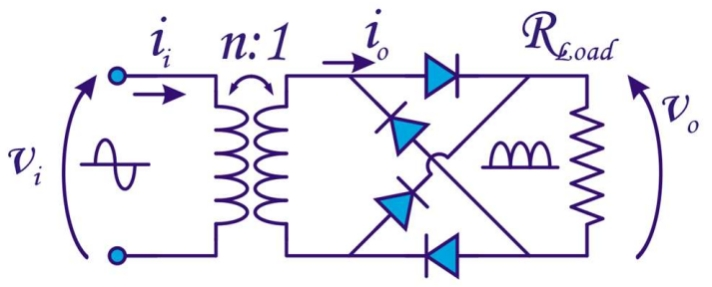
\includegraphics[width=8cm]{figures/ch12/graetz.jpg}
	\caption{}
	\label{fig:graetz}
\end{figure}

We see that the output voltage still has a very high ripple as in figure \ref{fig:dc_source4}, which can be (partially) removed with a low-pass filter. Because the signal has been rectified, the frequency has doubled: if the AC signal is 50 Hz, the cut-off frequency $f_c \approx 100$ Hz. An example is the use of a simple $RC$-filter as in figure \ref{fig:dc_source3}

\begin{minipage}{.5\textwidth}
	\centering
	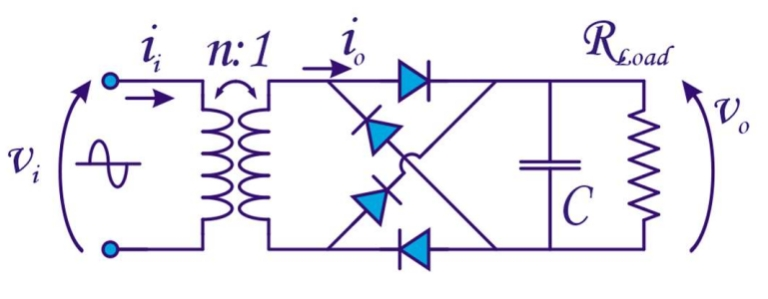
\includegraphics[width=8cm]{figures/ch12/dc_source3.jpg}
	\captionof{figure}{}
	\label{fig:dc_source3}
\end{minipage}%
\begin{minipage}{.5\textwidth}
	\centering
	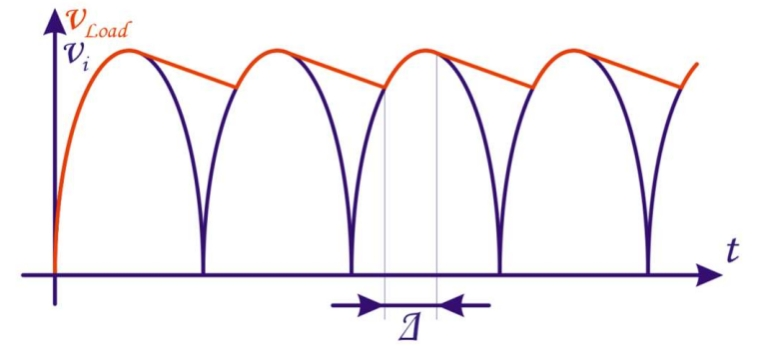
\includegraphics[width=6cm]{figures/ch12/dc_source4.jpg}
	\captionof{figure}{}
	\label{fig:dc_source4}
\end{minipage}

During the first part, where $v_i$ is increasing, the capacitor $C$ will charge until $v_i$ reaches a maximum. When $v_i$ will decrease, there is no more current through the top diode because with the capacitor charge, it is reversed biased. During that time, the capacitor will discharge through the load with a time constant $R_{Load} C$ which should be longer than half the period of the AC signal. 
So $v_{Load}$ decreases because $C$ discharges and $v_i$ increases during the second half period. When $v_{Load} = v_i$, the capacitor will start to charge again until $v_i$ reaches an optimum (a minimum in this case, but because of the rectification through the other diode it is seen by the load as a maximum) and the whole process starts again. The period during which the capacitor charges is called $\Delta$. This is also the only time when the diode conducts. During the other part of the cycle, the capacitor will provide the current to the load.\\
This also means that when the load  $R_{Load}$ receives an average current $I_{CC}$ during a period $T$, the total displaced charge is $Q_{Load} = I_{CC} T$. But this charge has to be provided by the diode during a time $\Delta$. So:
$$
Q_{Load} = I_{CC} T = I_{Diode} \Delta
$$
which means that $I_{Diode} = I_{CC} \frac{T}{\Delta}$. Consequently, if we try to make the ripple $e$ small, e.g. by choosing a large $C$, the charge period $\Delta$ will become small and the diode peak current will be very high, which can damage the diode. This means that a ripple can never be completely removed in the rectifier.


\section{Voltage Stabilizer}
\label{sec:voltage_stabilizer}
To further reduce the ripple, we can use a voltage stabilizer. This circuit will generate a DC voltage based on a reference, typically a Zener diode although sometimes we can use an integrated reference based on more advanced transistor effects.\\
The principle is shown in figure \ref{fig:stabilizer1}. The input is an average voltage $V_{IN}$, perturbed by a ripple $v_{in}$. We will always choose the Zener voltage $V_Z$ of the diode such that $V_{IN} + v_{in} > V_Z$. This diode is reversed biased and so the voltage seen by the load is $V_Z$, i.e we cut everything off above $V_Z$. Effectively, we remove the difference between $v_{IN}$ and $V_Z$, i.e. the voltage loss is $v_ {IN} - V_Z$. This is the loss over resistor $R$, such that the power loss through $R$ equals:
$$
P_R = \frac{(v_{IN} - V_Z)^2}{R}
$$
\begin{minipage}{.5\textwidth}
	\centering
	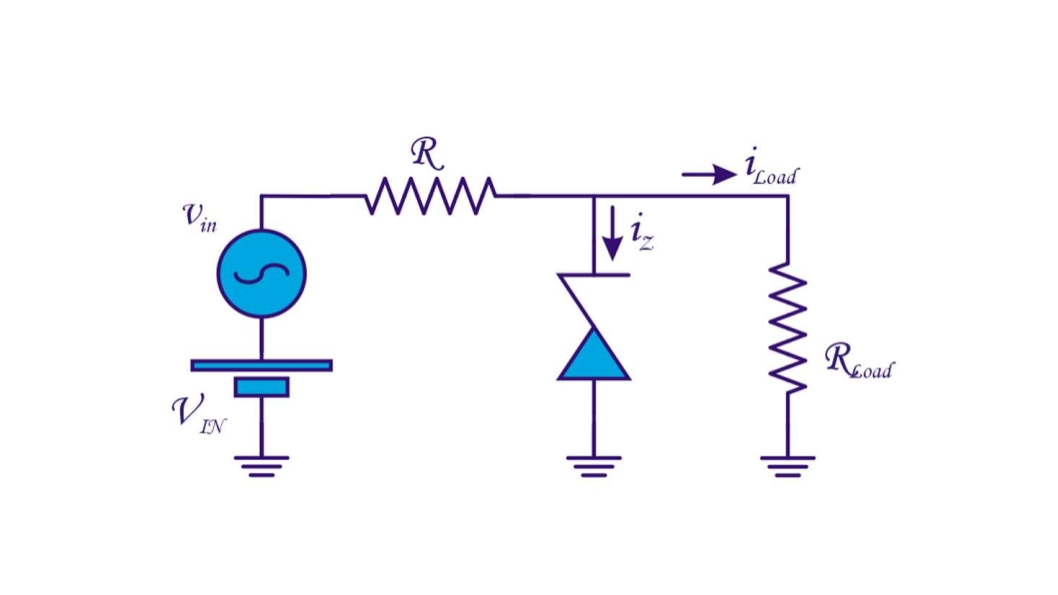
\includegraphics[width=8cm]{figures/ch12/stabilizer1.jpg}
	\captionof{figure}{}
	\label{fig:stabilizer1}
\end{minipage}%
\begin{minipage}{.5\textwidth}
	\centering
	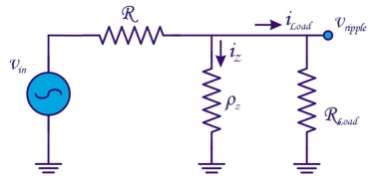
\includegraphics[width=6cm]{figures/ch12/stabilizer3.jpg}
	\captionof{figure}{}
	\label{fig:stabilizer3}
\end{minipage}
Because the power loss is inversely proportional to $R$, these resistors are normally relatively large and possibly cooled.\\
The diode load line can be calculated as:
\begin{align*}
	v_{IN} - v_Z = R\; (i_{Load} + i_Z) &= R \; \big( \frac{v_Z}{R_{Load}} + i_Z) \\
	\Rightarrow  \bigg(1 + \frac{R}{R_{Load}} \bigg) v_Z &= v_{IN} - i_Z R
\end{align*}
This load in figure  line is the green line \ref{fig:stabilizer2}, that goes through
$$(v_Z =  \frac{R_{Load}}{R_{Load} + R} v_{IN},\; i_Z = 0)  \text{ and } (v_Z = 0,\; i_Z = \frac{v_{IN}}{R})$$
The intersection of this line with the red Zener diode characteristic gives the operating point $Q$. This operating point must lie above the hyperbole of maximum power dissipation for the diode, determined by $V_D \; I_D  = P_{max}$. Note that the operating point $Q$ moves when $v_{IN}$ changes: when $v_{IN}$ is too large the diode will burn, when $v_{IN}$ becomes to small we'll leave the Zener region.
There are two types of external variations:
\begin{itemize}
	\item With constant $R_{Load}$, the current through the load is constant: $i_{Load} = \frac{V_Z}{R_{Load}}$. Any variation in $v_{IN}$ leads to a change in current through $R$ and this change has to be absorbed by the Zener diode.
	\item With a constant $v_{IN}$, the current through $R$ is constant: $i_R = \frac{v_{IN} - V_Z}{R}$. If $R_{Load}$ changes, the current through the load changes, and it is again the Zener diode who has to absorb this variation.
\end{itemize}

\begin{figure}[h!]
	\centering
	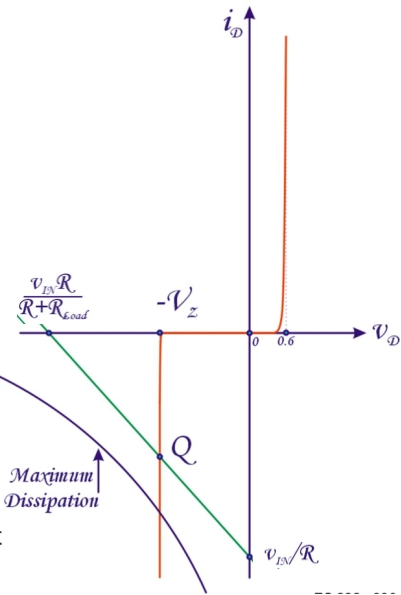
\includegraphics[height=8cm]{figures/ch12/stabilizer2.jpg}
	\caption{}
	\label{fig:stabilizer2}
\end{figure}
These variations can be computed by using the AC-equivalent circuit in figure \ref{fig:stabilizer3}. The Zener current varies:
\begin{itemize}
	\item With the input voltage: $i_z = \frac{v_{in}}{R}$,
	\item With the load voltage (assuming $v_{in} = 0$, i.e. $v_{IN}$ is constant): $i_z = -i_{load}$
\end{itemize}
This is difficult to control and during normal operation, the diode is likely to exit the Zener domain.\\
The residual ripple at the output can be obtained with:
$$\frac{v_{ripple}}{v_{in}} = \frac{\rho_z || R_{Load}}{R + \rho_z || R_{Load}} \approx \frac{\rho_z}{R + \rho_z}  \approx \frac{\rho_z}{R}$$
and this is small because $\rho_z$ is a very small resistance ($\sim \Omega$).
The output impedance is $R_{out} = \rho_z || R_{Load} || R \approx  \rho_z$.

\subsection{Double Stabilizer}

To avoid the difficulty with controlling the operating point, we can use the circuit in figure \ref{fig:stabilizer4}. This circuit isolates the input voltage $v_{in}$ from the load $R_{Load}$ because the current though resistor $R_2$ is fixed and determined by the difference in Zener voltages:
$$
i_{R2} = \frac{v_{Z1} - v_{Z2}}{R_2}
$$

\begin{figure}[h!]
	\centering
	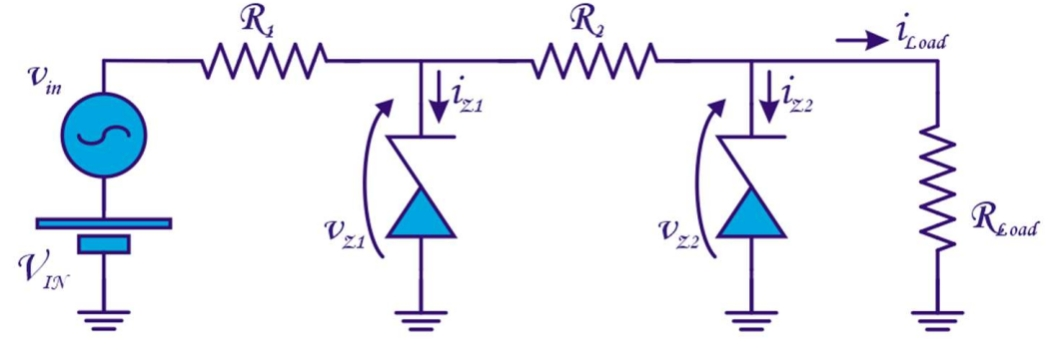
\includegraphics[width=10cm]{figures/ch12/stabilizer4.jpg}
	\caption{}
	\label{fig:stabilizer4}
\end{figure}

As a consequence, diode $D_1$ now absorbs the input voltage variation $v_{in}$: $i_{z1} = \frac{v_{in}}{R_1}$ and diode $D_2$ absorbs load variations: $i_{z2} = -i_{load}$.\\
The small-signal circuit of figure \ref{fig:stabilizer5} allows to compute the ripple. 
%We simplify a bit by assuming that the ripple at the output can be computed by a voltage divider consisting of $R_2$ and $\rho_{Z2} || R_{Load}$, and the ripple at $D_1$ is just $\frac{\rho_{Z1}}{R_1 + \rho_{Z1}} v_{in}$, i.e. the second part of the circuit doesn't load the first one. Then we can write:
By transforming $v_{in}$, $R_1$ and $\rho_{Z1}$ to the Thevenin equivalent with $v_{th} = \frac{\rho_{Z1}}{\rho_{Z1} + R_1} v_{in}$ and $Z_{th} = \rho_{Z1} || R_1$, we find:
\begin{align*}
	\frac{v_{ripple}}{v_{in}} &\approx \frac{\rho_{Z1}}{R_1 + \rho_{Z1}}  \frac{\rho_{Z2} || R_{Load}}{\rho_{Z2} || R_{Load} + R_2 + \rho_{Z1} || R_1} \\
							  &\approx \frac{\rho_{Z1} \rho_{Z2}}{R_1  R_2}
\end{align*}
So in addition to obtaining a more stable operating point, the ripple is significantly reduced. But note that there is an additional voltage and power loss over resistor $R_2$, because $V_{Z1}$ has to be larger than $V_{Z2}$.\\
Additionally, a good diode can handle currents of a couple mA, but not much more. We need another solution for loads that require more current, or for cases where the load (and hence the required current) is unknown. That's where we can use a transistor-based stabilizer.
\begin{figure}[h!]
	\centering
	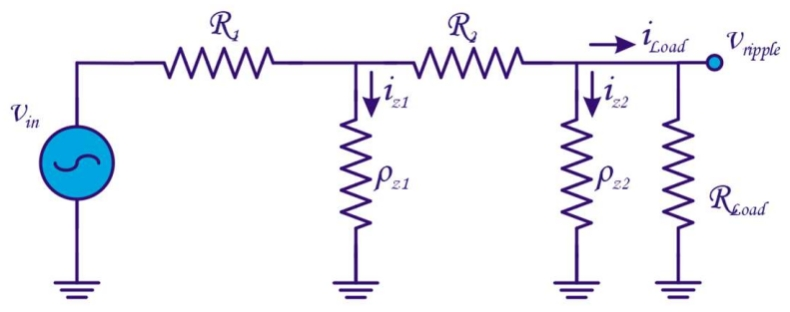
\includegraphics[width=10cm]{figures/ch12/stabilizer5.jpg}
	\caption{}
	\label{fig:stabilizer5}
\end{figure}

\subsection{Transistor-based Stabilizer}
\label{sec:transistor_stabilizer}
This stabilizer with transistor is an example of a series-stabilizer: the stabilizer is in series with the load. The Zener-diode keeps the base of the transistor at a fixed voltage $V_Z$, and the voltage at the load is equal to $V_Z - V_{BEQ}$. Hence the current through the load, and consequently also the $I_{CQ}$ of the transistor, is equal to $i_{load} = \frac{v_Z - V_{BEQ}}{R_{Load}}$
\begin{figure}[h!]
	\centering
	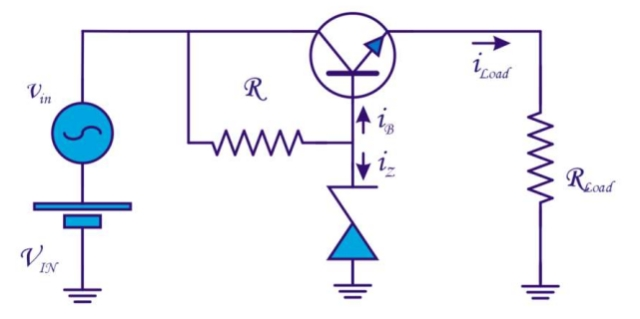
\includegraphics[width=10cm]{figures/ch12/stabilizer6.jpg}
	\caption{}
	\label{fig:stabilizer6}
\end{figure}

The voltage provided to load is set by the Zener-diode with the base-emitter junction of the transistor, i.e. $= V_Z - V_{BEQ}$. The transistor has to able to dissipate a power $P_T$:
\begin{align*}
	P_T = v_{CE} \; i_{load} = (v_{IN} - (v_Z - V_{BEQ})) \frac{v_Z - V_{BEQ}}{R_{Load}}
\end{align*}
which can be high.\\
Because the voltage at the transistor base is fixed, the current $i_R$ through resistor $R$ only varies with $v_{in}$. When $i_{Load}$ remains constant (i.e. the load doesn't change) the base current $i_B$ is also constant and all the variations of $i_R$ are completely absorbed by the diode. So: 
$$ i_z = \frac{v_{in}}{R}$$
The base current $i_B$ only depends on $i_{Load}: i_B =  i_{Load}/\beta$. So when $v_{in}$ remains constant and there is no current variation through $R$, $i_z$ has to vary with $i_{Load}$:
$$
i_z = -\frac{i_{Load}}{\beta}
$$
Once again, $i_z$ depends on both $v_{in}$ and $R_{Load}$, which is not ideal. However, because of the factor $\beta$, the variations due to the load are under control. Note how current variations of a couple of ampères are possible.\\
To compute the ripple and output impedance, we should draw the AC equivalent circuit. But we can redraw the circuit as in figure \ref{fig:stabilizer7} and note that this is a common-collector amplifier.\\
\begin{figure}[h!]
	\centering
	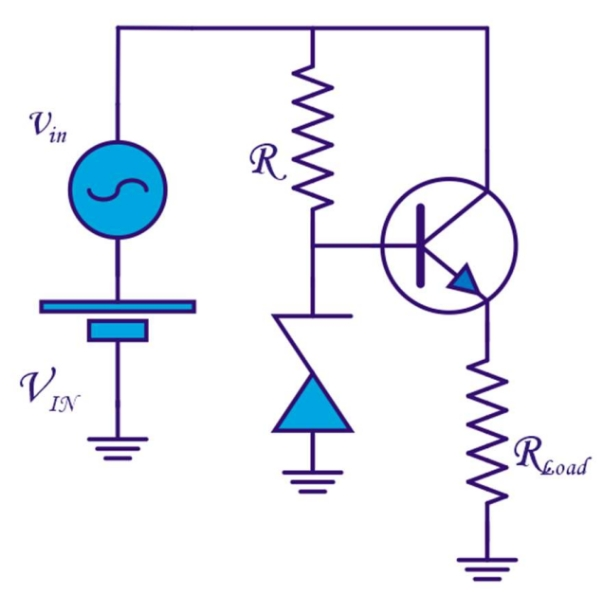
\includegraphics[width=6cm]{figures/ch12/stabilizer7.jpg}
	\caption{}
	\label{fig:stabilizer7}
\end{figure}
The output impedance is obtained by looking into the emitter of the transistor, so $R_{out} \approx \frac{1}{g}$. For the ripple, we see that the output at the emitter follows the base voltage variations, and this variation in turn is, for small signals, determined by the voltage divider formed by $R$ and $\rho_Z$:
$$
\frac{v_{ripple}}{v_{in}} = \frac{\rho_Z}{\rho_Z + R} \approx \frac{\rho_Z}{R}
$$
just as we found for the stabilizer with a single Zener-diode.\\
One way to isolate the reference diode from the load is with an operational amplifier in feedback, as in figure \ref{fig:stabilizer9}. The OPAMP will force the output voltage to be equal to voltage at its positive node, i.e. $V_Z$. For a fixed $v_{IN}$, the voltage drop across resistor $R$ is fixed and equal to $v_{IN} - V_Z$, and so is the current through $R$. So any variation in the load has no impact on  $i_Z$. The reference only suffers from a dependence of variations of $v_{IN}$: $i_z = \frac{v_{in}}{R}$.
\begin{figure}[h!]
	\centering
	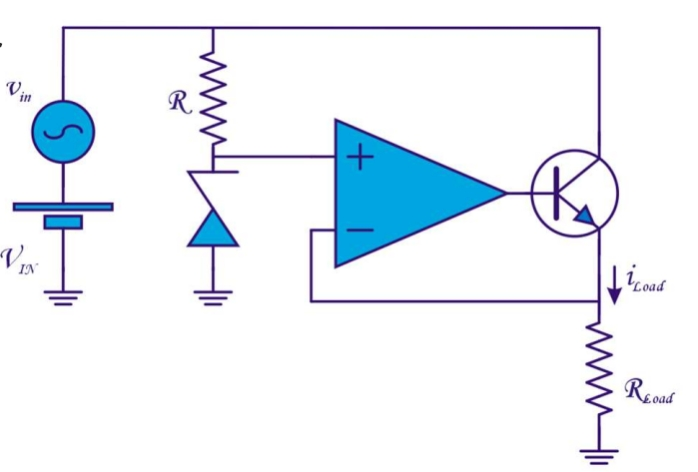
\includegraphics[width=10cm]{figures/ch12/stabilizer9.jpg}
	\caption{}
	\label{fig:stabilizer9}
\end{figure}
The ripple is like before determined by the voltage divider $R$ - $\rho_Z$: $\frac{v_{ripple}}{v_{in}} = \approx \frac{\rho_Z}{R}$. The output impedance as seen by the load is $R_{out} \approx \frac{1}{A_V g}$. This is because the impedance looking into the emitter is $\frac{1}{g}$, and feedback reduces the output impedance by a factor of about $A_v$ (see section \ref{sec:impedance_feedback}). The output impedance is thus extremely low.

\section{Supply Protection}

The goal of a supply protection is to avoid that a load will draw too much current from the DC supply: this could cause damage to the circuitry. We could use a fuse, but this is in general slow, and it might happen that part of the circuit already has been damaged before the fuse has molten. So we typically rely on electronic circuitry that acts fast and saves the circuit. There are two types of protection:
\begin{itemize}
	\item A \emph{current limiter}, as in figure \ref{fig:supply_prot1}. If the current exceeds a certain threshold $i_{max}$, the circuit shuts down: there is still current, but the supplied voltage becomes zero.
	\item A \emph{current fall-back} circuit (figure \ref{fig:supply_prot2}) that shuts both current and supply voltage down and reduces them to zero. This is much better than a current limiter, but requires a reset to restore proper operation.
\end{itemize}

\begin{minipage}{.5\textwidth}
	\centering
	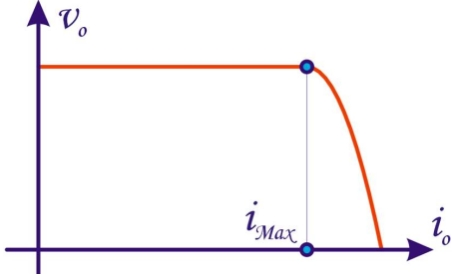
\includegraphics[width=6cm]{figures/ch12/supply_prot1.jpg}
	\captionof{figure}{}
	\label{fig:supply_prot1}
\end{minipage}%
\begin{minipage}{.5\textwidth}
	\centering
	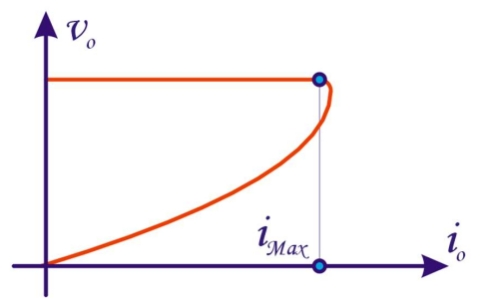
\includegraphics[width=6cm]{figures/ch12/supply_prot2.jpg}
	\captionof{figure}{}
	\label{fig:supply_prot2}
\end{minipage}

We will examine how a current limiter can be implemented. Consider the circuit in figure \ref{fig:supply_prot3}. This is the improved output stage of figure \ref{fig:stabilizer9}. The voltage $V_{ref}$ is generated by a Zener diode. The resistor $R$ is chosen such that $I_{max} = \frac{V_{BEQ}}{R}$. For a small load current, the bottom transistor is blocked and the top transistor provides the current, just as in figure \ref{fig:stabilizer9}. The OPAMP sets the output current to $V_{ref}$.

\begin{figure}[h!]
	\centering
	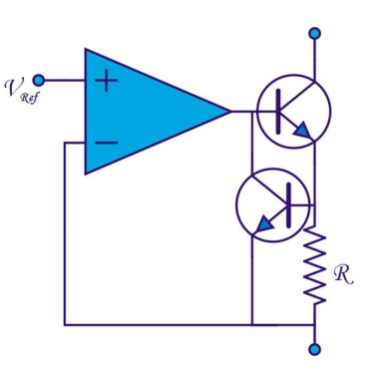
\includegraphics[width=6cm]{figures/ch12/supply_prot3.jpg}
	\caption{}
	\label{fig:supply_prot3}
\end{figure}

As the current increases, so will the voltage drop over $R$. When the current reaches $I_{max}$, the bottom transistor has enough base-emitter voltage and it starts to conduct. It will steal base current from the top transistor and any additional current can no longer be provided by this transistor. If there is current beyond $I_{max}$, it has to come from the OPAMP. But the OPAMP is a voltage amplifier, and is not equipped to provide much current. The OPAMP will no longer be able to supply the required current and breaks down, which causes the output voltage to drop to zero.

\section{Switched Supply}

PM